\chapter{PID design using frequency response}

In this lab, you will use the Bode plot you produced using the measurements
for the motor to design a PID controller to meet specified performance
criteria.

\section{Prelab}

Before you go into the lab, you should read the following:
\begin{itemize}
\item Section 12.2 from the course text on using
frequency response method for controller design.
\end{itemize}
Since \textsf{Simulink} does not allow improper transfer functions, you must
use the \verb|PID| block for the controller in this lab.  Find the
relationships between the constants in equation~\eqref{eqn:con1}
and~\eqref{eqn:con2}\@:
\begin{gather}\label{eqn:con1}
\frac{K}{s}(1+T_{D}s)(s+\frac{1}{T_{I}}),\\\label{eqn:con2}
P+\frac{I}{s}+Ds.
\end{gather}

\section{Procedure}

Before we implement the controller, we need to do some paper work to design
it.

\subsection{Design specifications}

You are charged with the designing the controller rational function $R_{C}$
in the feed back loop in Figure~\ref{fig:PIDfeedback}\@.
\begin{figure}[htbp]
\centering
\begin{picture}(230,75)
\put(0,50){\(\hat u(s)\)}
\put(20,53){\vector(1,0){15}}
\put(40,53){\circle{7}}
\put(28,57){+}
\put(45,53){\vector(1,0){20}}
\put(68,37){\framebox(35,33){\normalsize \(R_{C}(s)\)}}%-50 in width
\put(105,53){\vector(1,0){40}}
\put(147,37){\framebox(35,33){\normalsize \(R_{P}(s)\)}}
\put(185,53){\vector(1,0){30}}
\put(217,50){\(\hat y(s)\)}
\put(201,53){\line(0,-1){45}}
\put(201,8){\line(-1,0){161}}
\put(40,8){\vector(0,1){40}}
\put(30,48){\line (1,0) {4}}
\end{picture}
\caption{Feedback system with disturbance}\label{fig:PIDfeedback}
\end{figure}%
The plant transfer function is that for the motor:
\begin{equation*}
R_{P}(s)=\frac{k_{E}}{s(s+\frac{1}{\tau})},
\end{equation*}
where you have measured the values for $k_{E}$ and $\tau$ in Lab~\ref{chap:intro}\@.

You are asked to design a controller so that the closed-loop system has a
phase margin of $65^{\circ}$ and a crossover frequency as large as possible.
The controller you will use is a PID controller in the form
\begin{equation*}
R_{C}(s)=\frac{K}{s}(1+T_{D}s)(s+\frac{1}{T_{I}})=
K(1+\frac{T_{D}}{T_{I}}+T_{D}s+\frac{1}{T_{I}s}).
\end{equation*}

\subsection{The steps in controller design}

We shall lead you by hand through the design process.
\begin{enumerate}
\item Produce the Bode plot for plant transfer function using
\textsf{Matlab}.

\item In the PID controller design, let us decide to fix $T_{I}=10T_{D}$\@.
You are free to change this ratio during the lab if you find it unsuitable.

\item Also, to start the design process, let us fix the gain $K$ to 1.  You
may want to use the \verb|zpk| function in \textsf{Matlab} to define the
transfer function.

\item With the above assumptions, is it true that there is a choice for
$T_{D}$ for which the closed loop system is IBIBO stable (IBIBO stability can
be verified either by Nyquist Criterion or Hurwitz Criterion)?  Is it true
that, no matter what choice one makes for $T_{D}$\@, the closed-loop system
will be IBIBO stable?  Can you spot the features on your Bode and/or Nyquist
plot which help you answer this question?  How do these play a role in the
design of the controller?

\item Based upon the considerations in the previous step, choose a value for
$T_{D}$ which meets the design objectives.

\item Now choose $K$ to give the crossover frequency.

\item Make sure the closed-loop system is IBIBO stable using the Nyquist
criterion.
\end{enumerate}

You now have values for $K$\@, $T_{D}$\@, and $T_{I}$ which you will carry
into the rest of the procedure.

\subsection{Executing the design in hardware/software}

Now you will implement your controller in hardware.
\begin{enumerate}
\item Open \textsf{Matlab} and build a \textsf{Simulink} model according to
Figure~\ref{fig:model9a}\@.
\begin{figure}[htbp]
\centering
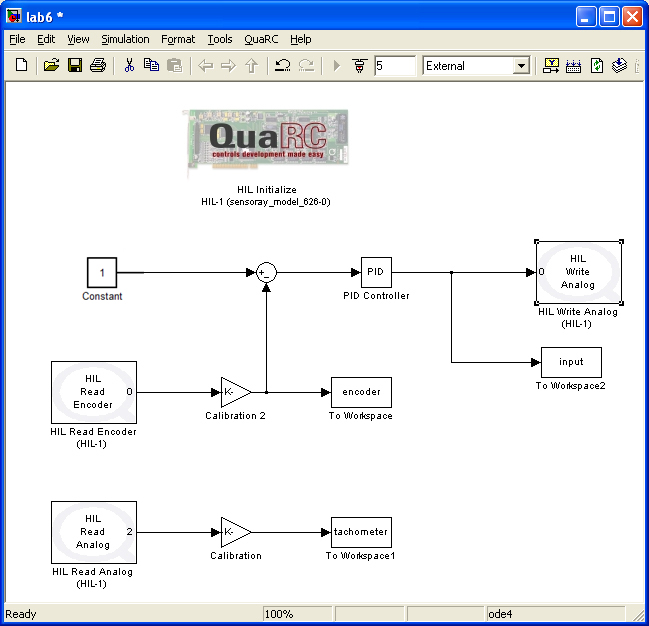
\includegraphics[width=0.6\hsize]{pix/lab9a.jpg}
\caption{\textsf{Simulink} model for the implementation of PID control using
frequency response method; step reference}\label{fig:model9a}
\end{figure}%

\item Use values for $K$\@, $T_D$\@, and $T_I$ that make the closed loop
system unstable in hardware.  Use the above contraints you just calculated to
determine values that cause instability.  Be prepare to shut the system off!
Produce plots of the unstable system.

\item Now, using an input step response of $1$\@, use the ``good'' values for
$K$\@, $T_D$\@, and $T_I$ to determine the rise time, the percentage
overshoot, and the $\epsilon$-settling time for $\epsilon=0.5$\@.

\item Now run the system with your ``good'' values for $K$\@, $T_D$\@, and
$T_I$ and a sinusoidal input whose magnitude is $1$ and whose frequency is
the crossover frequency that was calculated above; see
Figure~\ref{fig:model9} for the \textsf{Simulink}\@.
\begin{figure}[htbp]
\centering
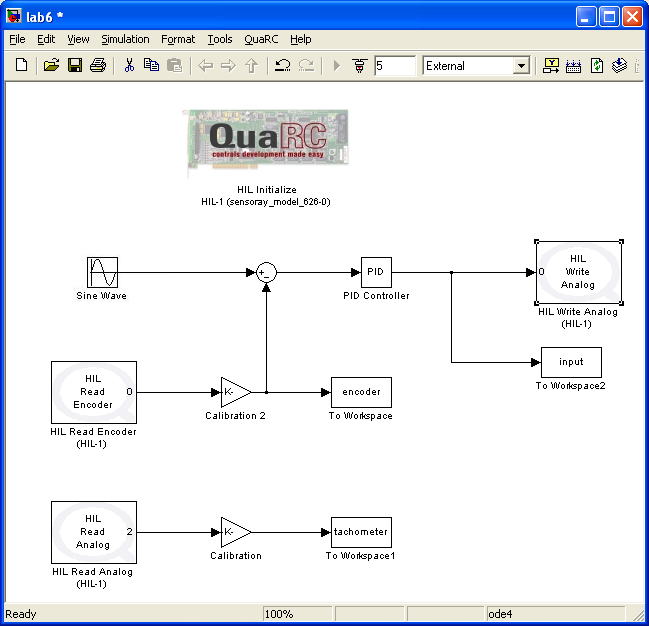
\includegraphics[width=0.6\hsize]{pix/lab9.jpg}
\caption{\textsf{Simulink} model for the implementation of PID control using
frequency response method; sinusoidal reference}\label{fig:model9}
\end{figure}%
What is the magnitude of the output compared to the input, and what is the
phase of the output relative to the input?

\item Is your controller a good one?  How might you improve it?  What do your
improvements mean in terms of loopshaping ideas?

\item Change the ratio of $\frac{T_{I}}{T_{D}}$ and discuss the effect on the
performance of the controller.  Does what you observe make sense?  Generate
plots to demonstrate your observations.
\end{enumerate}

When you have completed the lab, make sure you save your files in the folder
you created in Lab~\ref{chap:intro}\@.

%%% Local Variables: 
%%% mode: latex
%%% TeX-master: "lab-manual"
%%% End: 
